\chapter{Анализ физических данных эксперимента РЭД-100 на Калининской АЭС} 
\label{chapt4}
Для увеличения достоверности результатов, проводился так называемый слепой анализ. Все методы обработки и анализа в данном случае отрабатываются на фоновых данных (набранных при выключенном реакторе), и только после полного понимания всех процедур допускается их применение к данным, набранным со включенным реактором без изменений.
\section{Моделирование УКРН событий}
\label{sect4_1}
Важным этапом при анализе данных эксперимента является детальное понимание отклика детектора на сигнальные события. Для эксперимента РЭД-100 на КАЭС сигнальными событиями являются события от УКРН. 

Учитывая известную мощность реактора моделировался энергетический спектр ядер отдачи в GEANT-модели детектора, который далее пересчитывался в спектр, выраженный в электронах ионизации. При дрейфе и экстракции с поверхности электроны ионизации претерпевают потери, которые были рассчитаны с использованием полученных в \ref{sect3_1} и \ref{sect3_5} значений времени жизни электронов в жидком ксеноне и коэффициента экстракции, соответственно. Спектр до и после данных потерь представлен на рисунке \ref{img:cevnscpectrum}.
\begin{figure}[H]	
\center{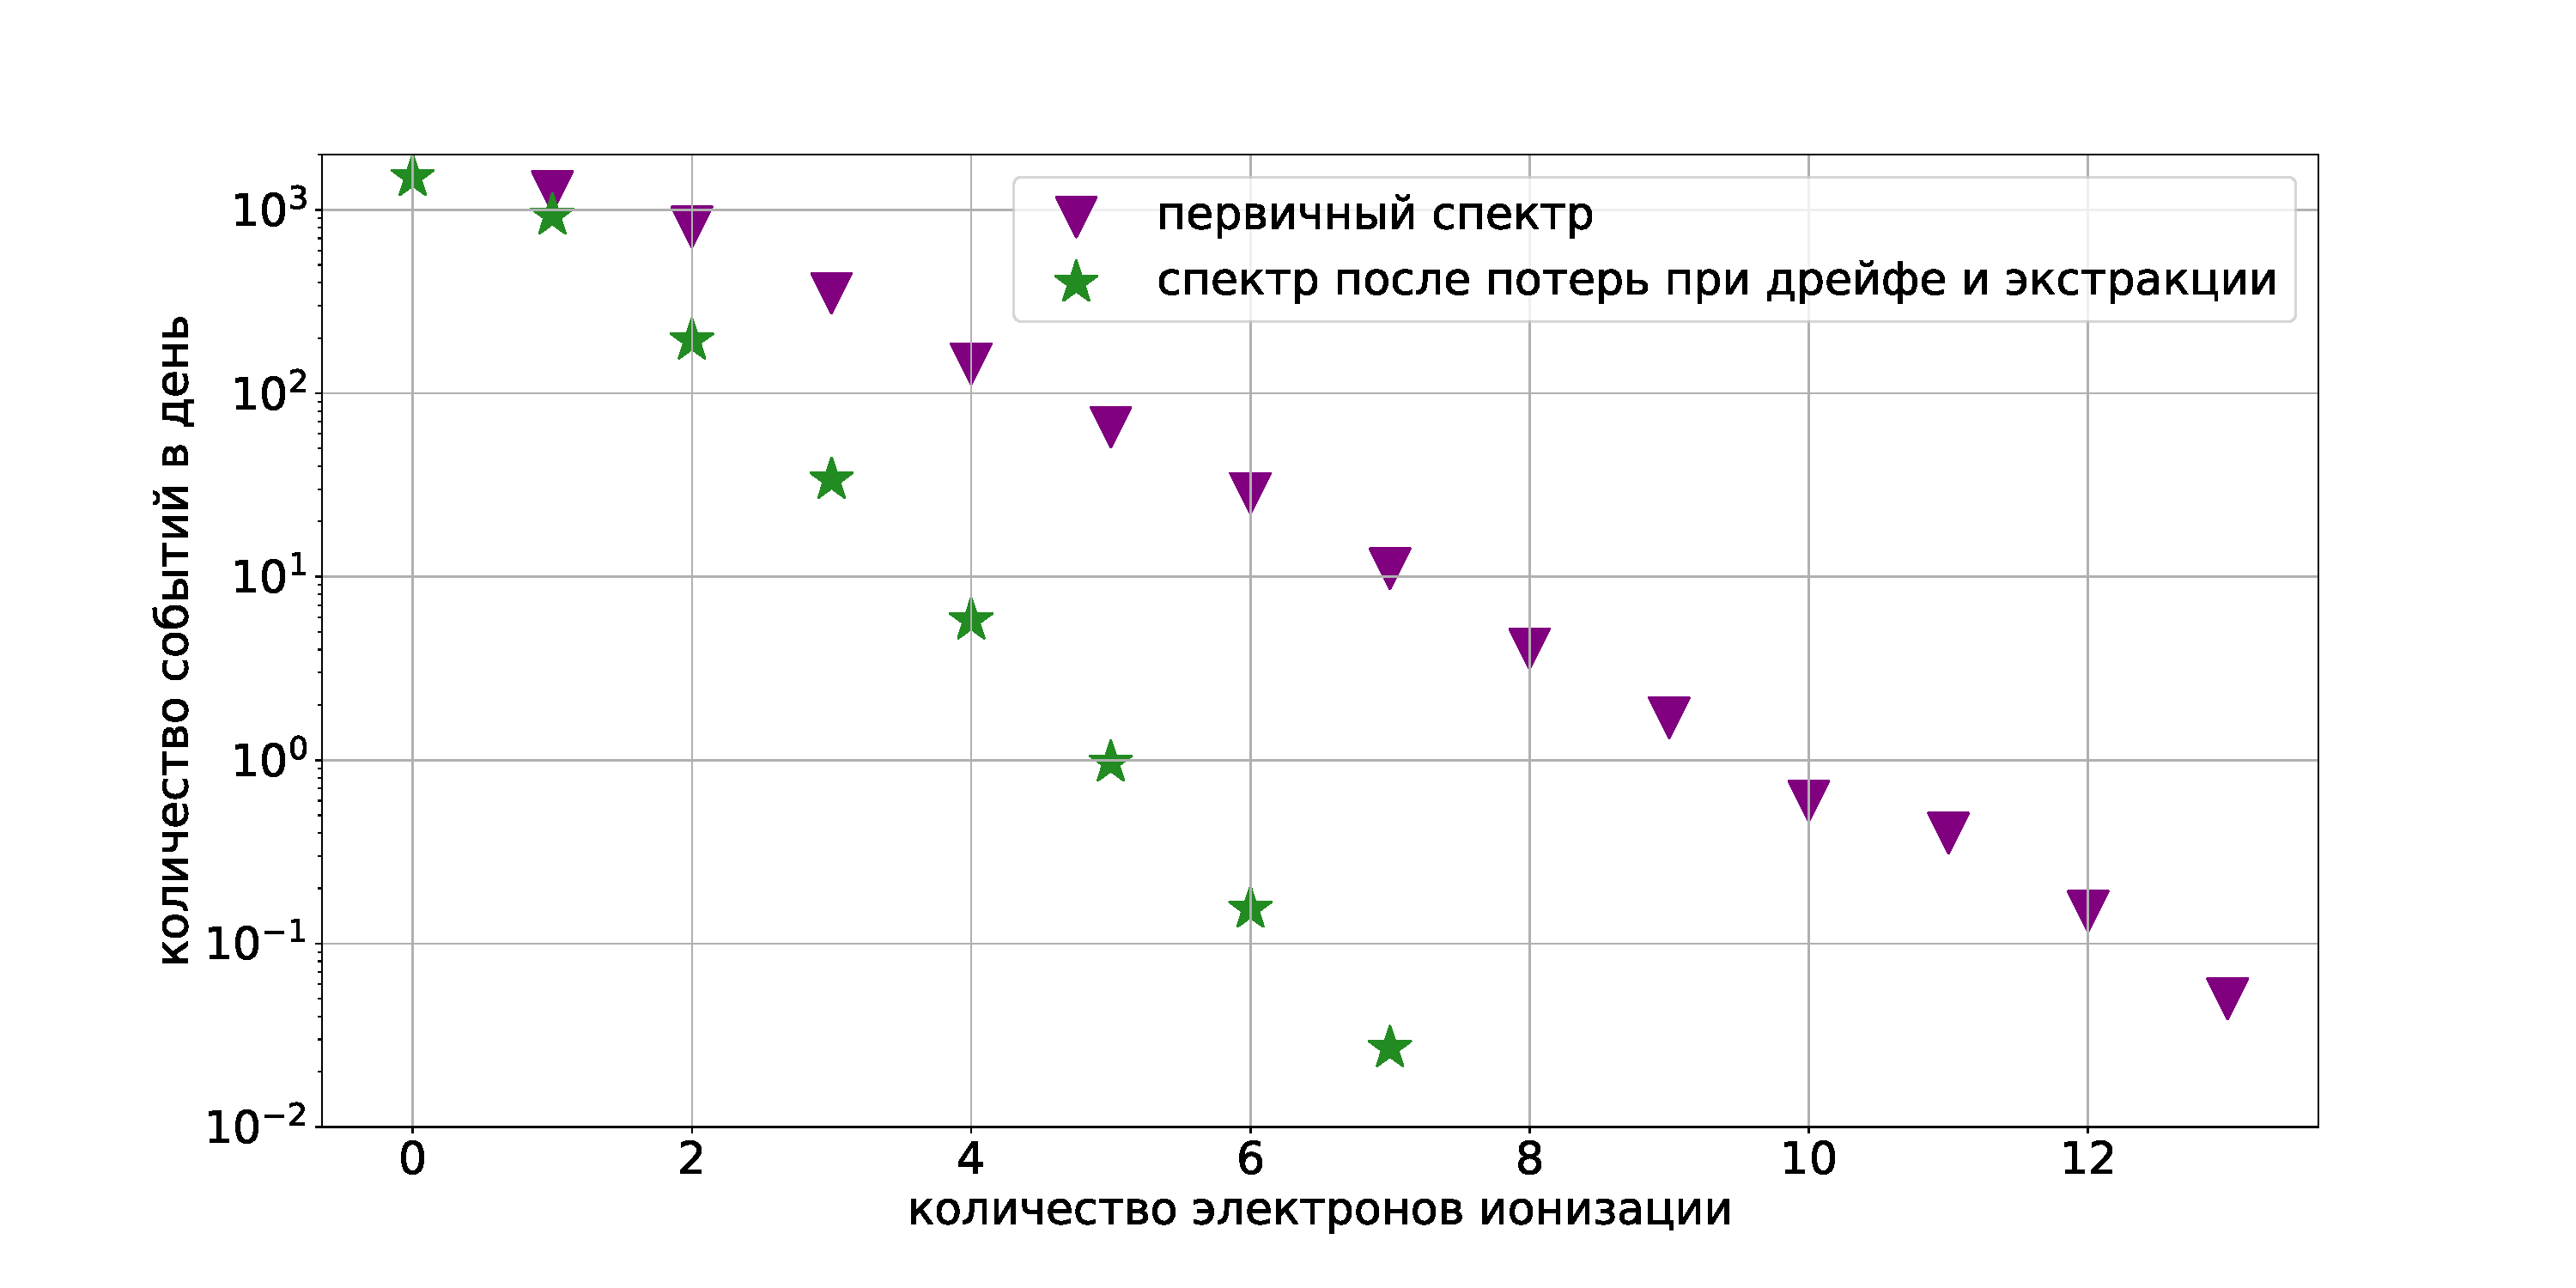
\includegraphics[width=1.0\linewidth]{images/cevnsspectrumSE.pdf}}
	\caption{Смоделированный спектр УКРН-событий, выраженный в электронах ионизации, до и после потерь при дрейфе и экстракции.}
	\label{img:cevnscpectrum}
\end{figure}

Далее, в соответствии с описанной в \ref{subsect2_3_2} процедурой были смоделированы события в несколько электронов ионизации согласно полученному спектру. При моделировании использовались LRF, полученные при анализе измерений с гамма-источниками. Также была проведена процедура реконструкции координат и энергии данных событий. Для улучшения соотношения сигнал/шум при дальнейшем анализе к событиям были применены дополнительные отборы по длительности (<5 мкс) и радиусу (<130 мм), совпадающие с отборами для экспериментальных данных. Результирующий спектр восстановленной энергии смоделированных УКРН-событий представлен на рисунке \ref{img:cevnscpectrumspe}. 
\begin{figure}[H]
\center{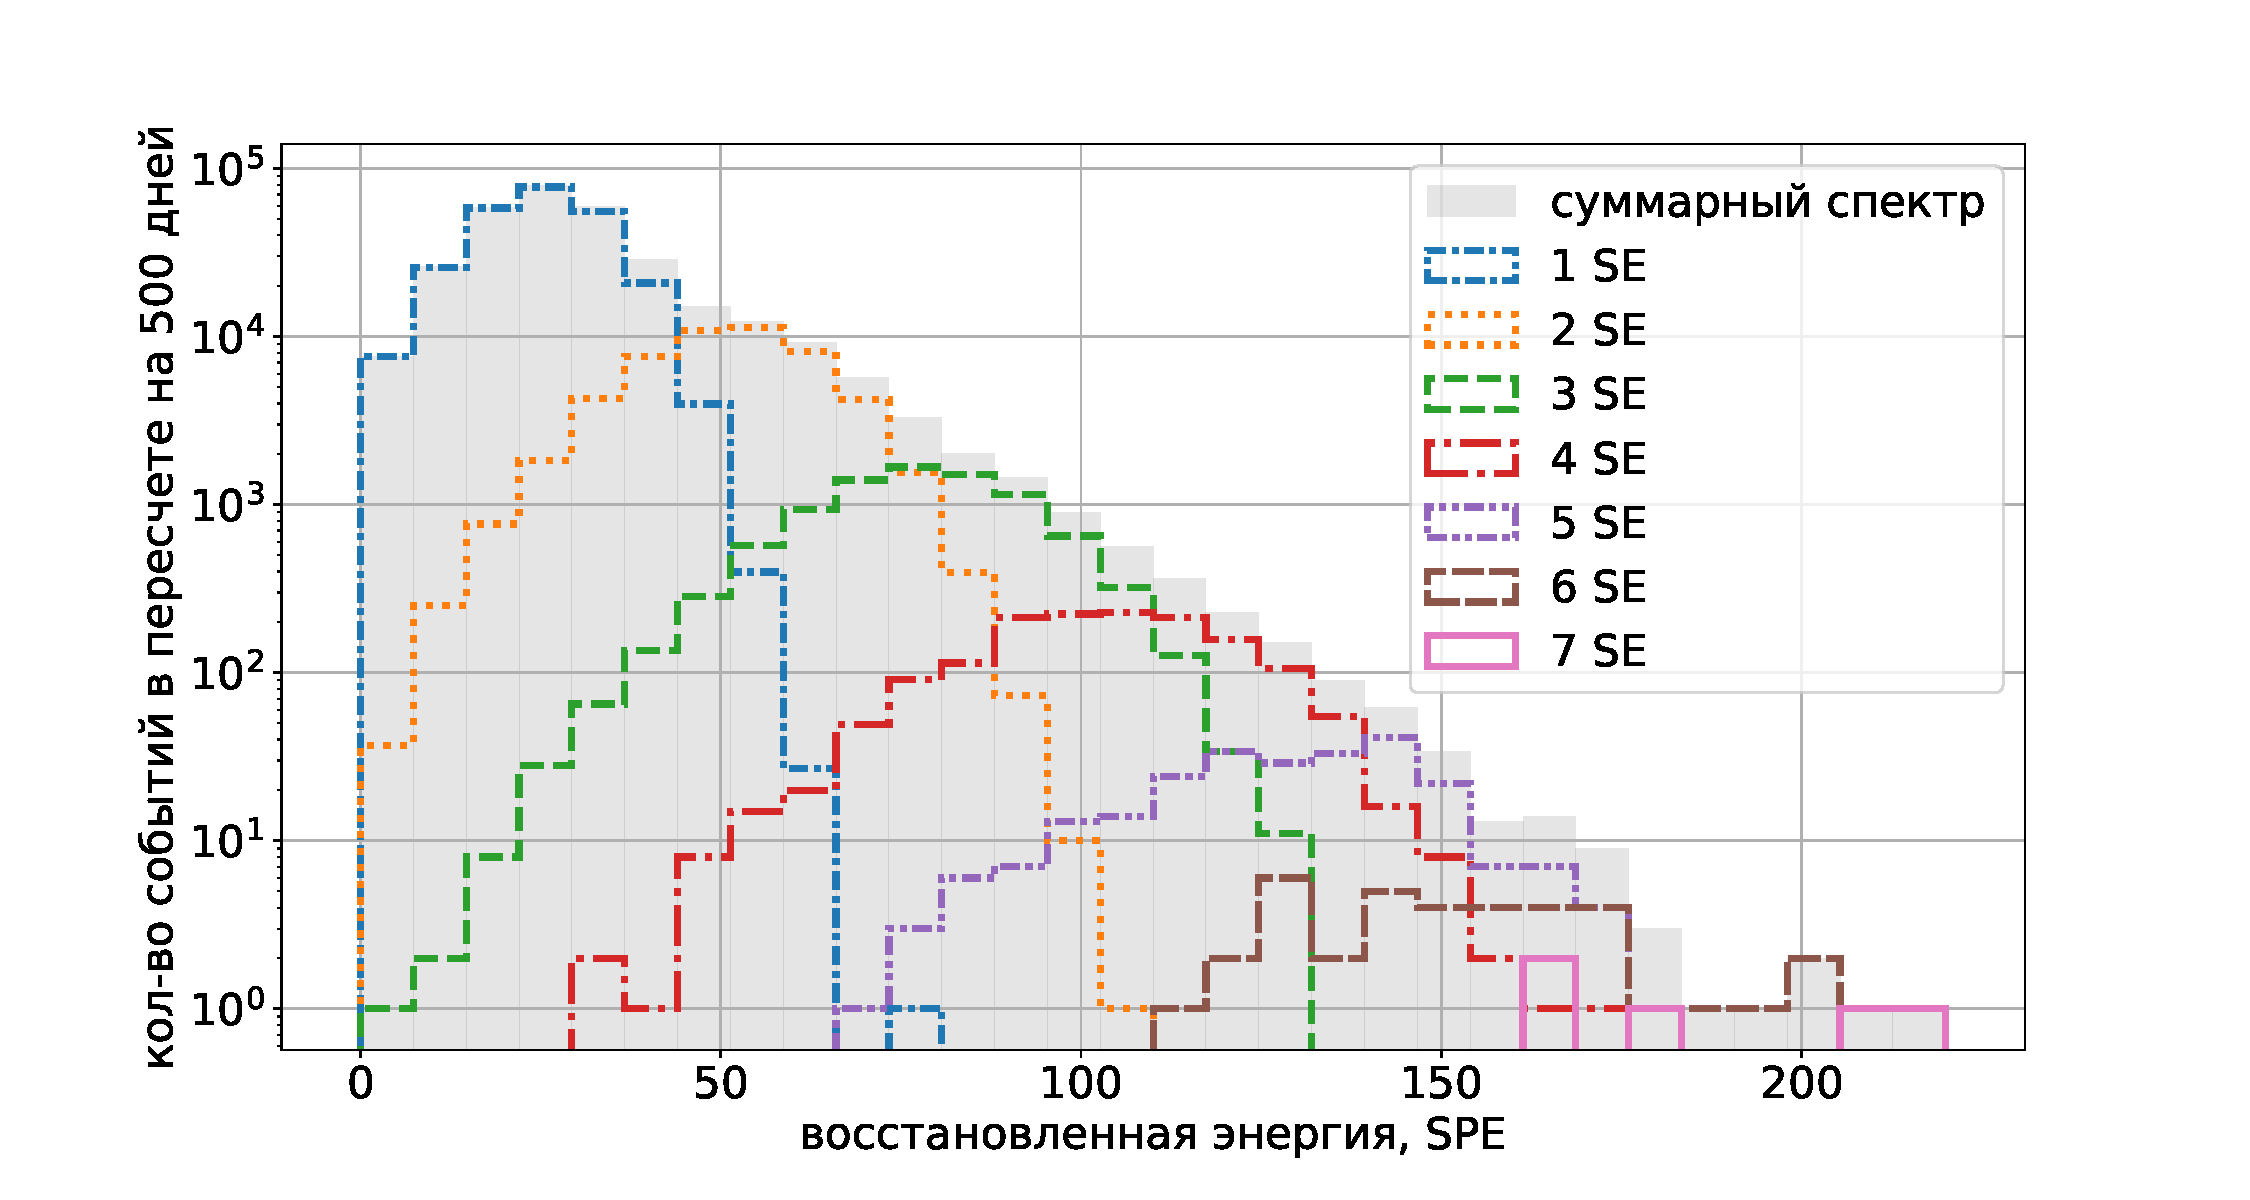
\includegraphics[width=1.0\linewidth]{images/cevnsspectrumSPE.pdf}}
	\caption{Спектр восстановленной энергии смоделирванных УКРН-событий.}
	\label{img:cevnscpectrumspe}
\end{figure}


\section{Кластеризация и отбор экспериментальных данных}
\label{sect4_2}
При наборе ME-данных использовался триггер, описанный в~\ref{subsect2_1_3}, позволяющий записывать события в несколько электронов ионизации. На записанных формах сигнала выделялись следующие диапазоны:
\begin{itemize}
    \itemОбласть перед триггером: от 0 до 15 мкс
    \itemОбласть триггера: от 17.5 до 20.5 мкс
    \itemОбласть после триггера: от 22 мкс до 30 мкс
\end{itemize}

Первичный отбор кластеров событий в несколько электронов ионизации (ME -- Multiple Electrons) аналогичен соответствующей процедуре для SE-событий (см~\ref{sect3_4}). Отличие заключалось в выборе пороговых значений для отбора импульсов, связанное с изменением SPE-калибровки. Таблица с пороговыми значениями представлена в~\ref{AppendixA3}. Кроме того, на события были наложены дополнительные отборы, учитывающие форму сигнала:
\begin{itemize}
    \item нет отсчетов, отклоняющихся в противоположную сигналу сторону более чем на 10~мВ (данный отбор обеспечивает защиту от так называемого "звона" в каналах)
    \item в кластере присутствует не менее 20 импульсов
    \item начало кластера находится в области триггера или начало находится до области триггера, а конец -- после
    \item для каждого импульса отношение характерного заряда SPE в соответствующем канале к амплитуде импульса больше порогового значения в 2.0 (данный отбор обеспечивает защиту от наличия высокоамплитудных одиночных импульсов, которые могут возникать как от сцинтилляции, так и от черенковского излучения)
    \item отношение суммарной площади импульсов в окрестности ([-20,+180]~нс) самого большого импульса кластере к полной сумме всех импульсов кластера меньше порогового значения 0.4 (цель данного отбора аналогична цели предыдущего)
    \item отношение площади импульсов внутри интервала длительностью 1 мкс, находящегося внутри кластера и дающего максимальный вклад в суммарную площадь, к общей площади импульсов кластера меньше порогового значения 0.84 (данный отбор позволяет бороться с событиями, внутри которых наблюдается существенное отклонение от равномерности распределения импульсов по времени внутри кластера)
    \item длительность кластера составляет от 1.6 до 5.0 мкс
    \item в области перед триггером находится менее 50 импульсов
    \item в области после триггера находится менее 35 импульсов
    \item восстановленный при помощи LRF радиус меньше 130~мм
\end{itemize}

Пример суммарной формы сигнала события, прошедшего все отборы, представлен на рисунке~\ref{img:event_example}.
\begin{figure}[H]
\center{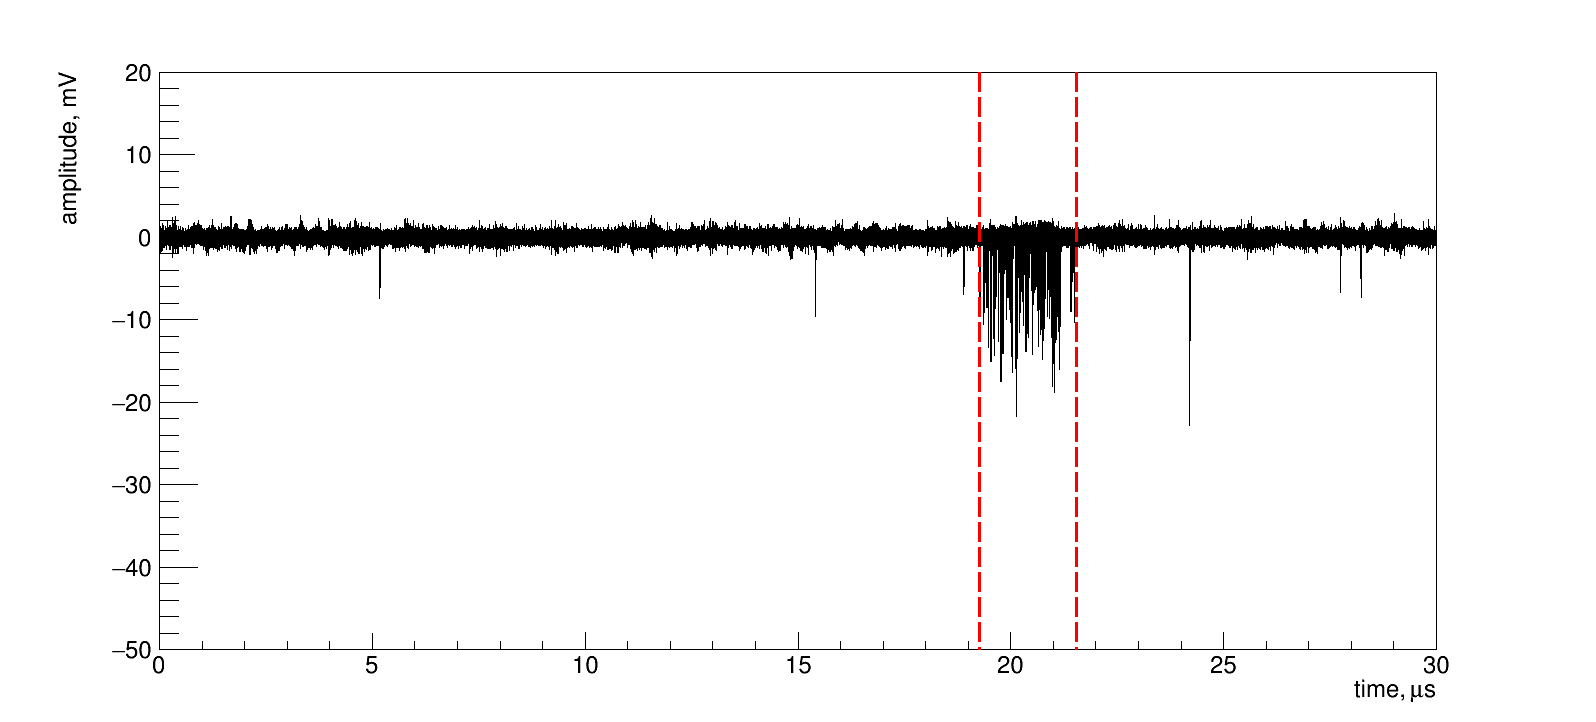
\includegraphics[width=0.8\linewidth]{images/pic_run0520_file0002_ev1049.png}}
	\caption{Пример суммарной формы сигнала события, прошедшего все отборы.}
	\label{img:event_example}
\end{figure}

Как уже упоминалось в \ref{subsect2_1_5}, существенную часть фона составляет совпадающие по времени сигналы от одного или нескольких спонтанно возникших электронов ионизации, как показано на рисунке~\ref{img:overlap}.
\begin{figure}[H]
\center{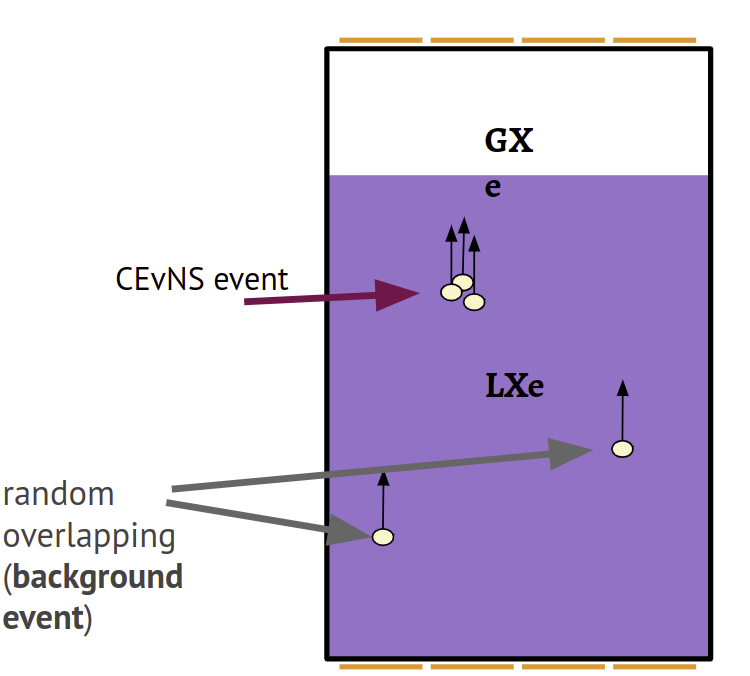
\includegraphics[width=0.5\linewidth]{images/randomoverlap.png}}
	\caption{Иллюстрация механизма возникновения событий совпадения.}
	\label{img:overlap}
\end{figure}

Для борьбы с такими событиями можно использовать идею о том, что точечные события не могут давать множественные вершины на плоскости XY. С целью подавления данной компоненты фона были применены технологии машинного обучения, а именно были разработаны две нейронные сети. Обучение сетей производилось на смоделированных событиях.
Точечные события для обучения нейронных сетей моделировались по такому же принципу, как и события УКРН. События совпадения конструировались из двух или более точечных событий, произошедших в одно время, но в разных местах на плоскости XY.

Первая нейронная сеть представляет собой полносвязный перцептрон~\cite{perceptron}, который в качестве входных данных использует только распределение света по верхней матрице ФЭУ, без учета времени возникновения сигналов.

Вторая нейронная сеть помимо полносвязных слоев имеет в своем составе сверточные~\cite{INDOLIA2018679} и принимает на вход псевдо-изображение 19х19 пикселей, где по вертикальной откладывался номер ФЭУ, а по горизонтальной оси -- время регистрации фотонов. Числовое значение в каждом пикселе соответствовало количеству зарегистрированных фотонов в конкретном канале в конкретный бин по времени. Примеры описанных выше изображений приведены на рисунке~\ref{img:cevnsbckgevents}. Анализ подобных псевдо-изображений применялся для восстановления координат и энергии в работе~\cite{Delaquis_2018}. 

Результаты отбора УКРН событий и подавления фона, расчитанные по смоделированным данным приведены в таблицах~\ref{NNeffcevns}~и~\ref{NNeffbckg}. Для дальнейшего анализа отбирались события, идентифицированные обеими сетями как точечные.

\begin{figure}[ht]
  \begin{minipage}[ht]{0.49\linewidth}    \center{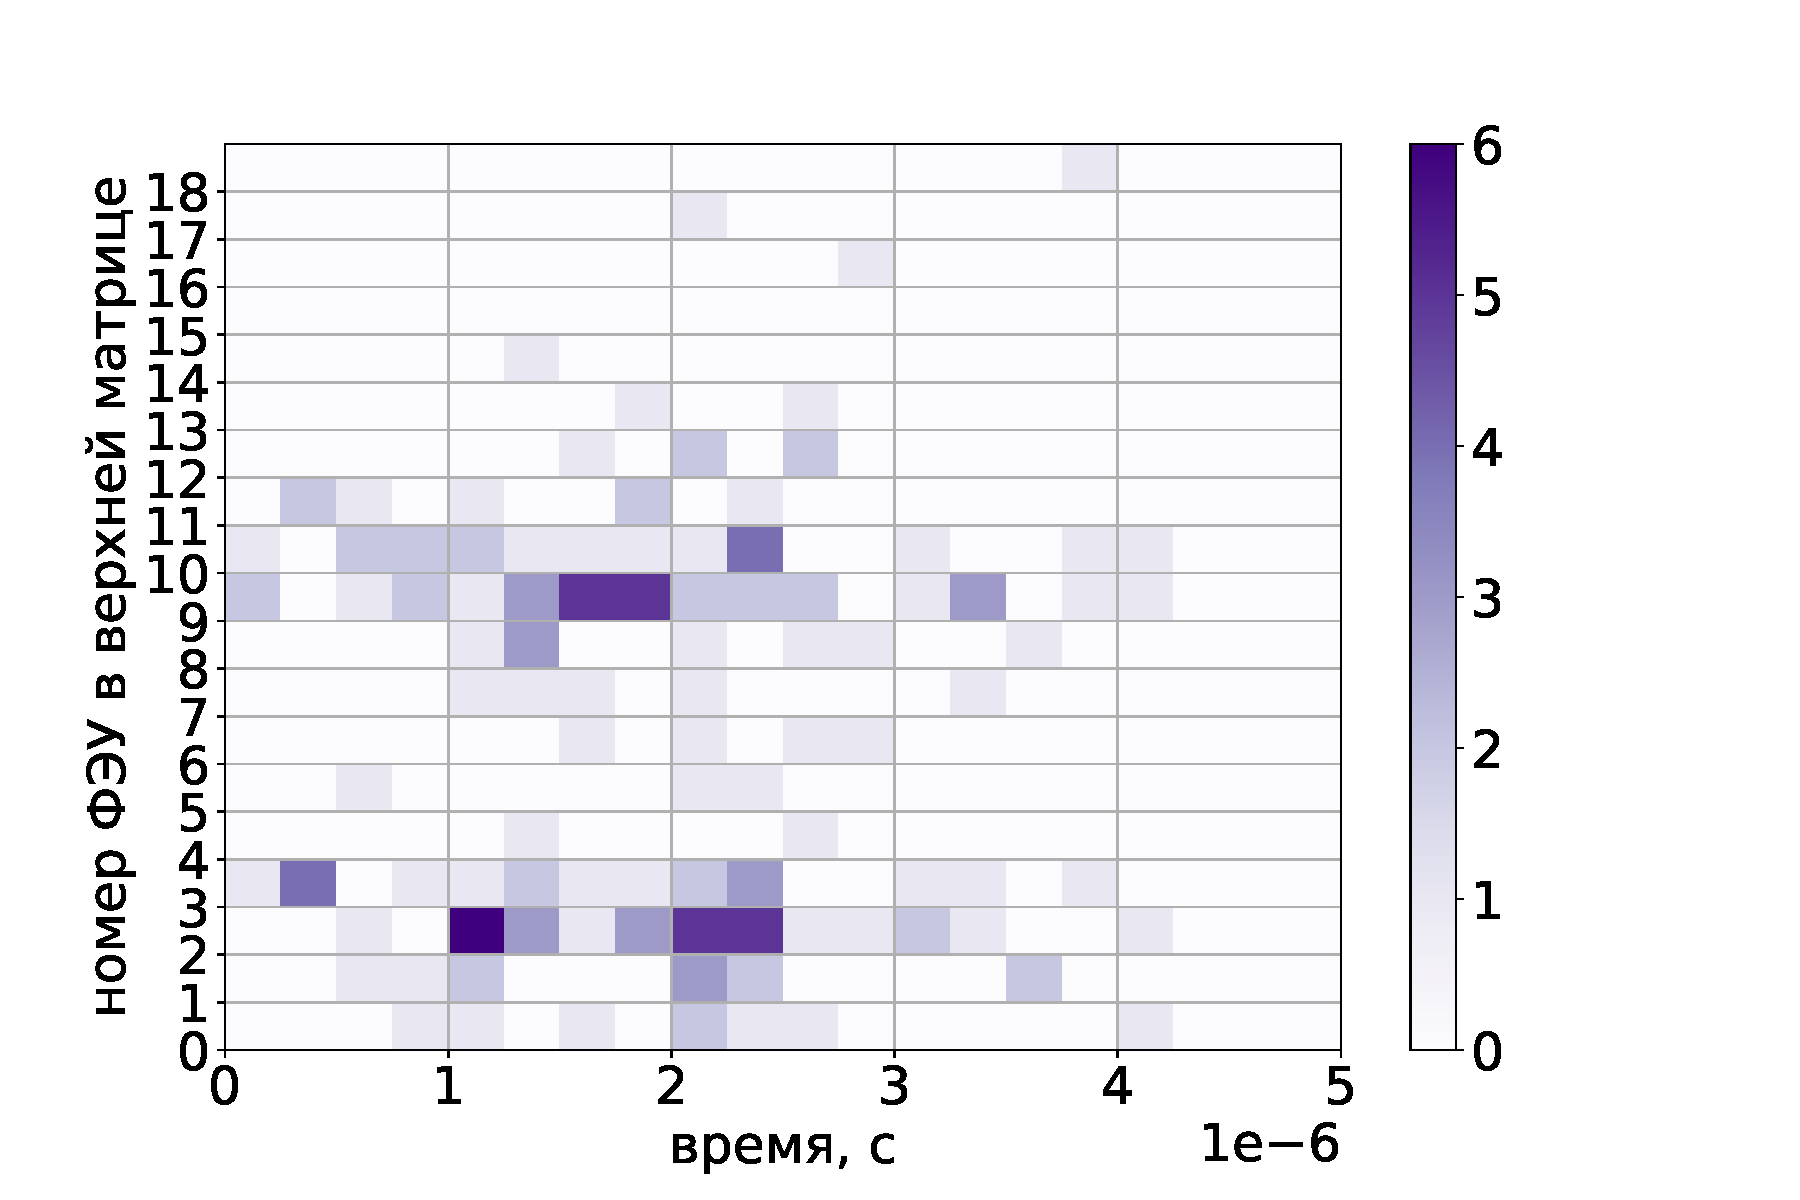
\includegraphics[width=1.0\linewidth]{images/cevns_event_6SE_1206_0.pdf} \\ а)}
  \end{minipage}
  \hfill
  \begin{minipage}[ht]{0.49\linewidth}  \center{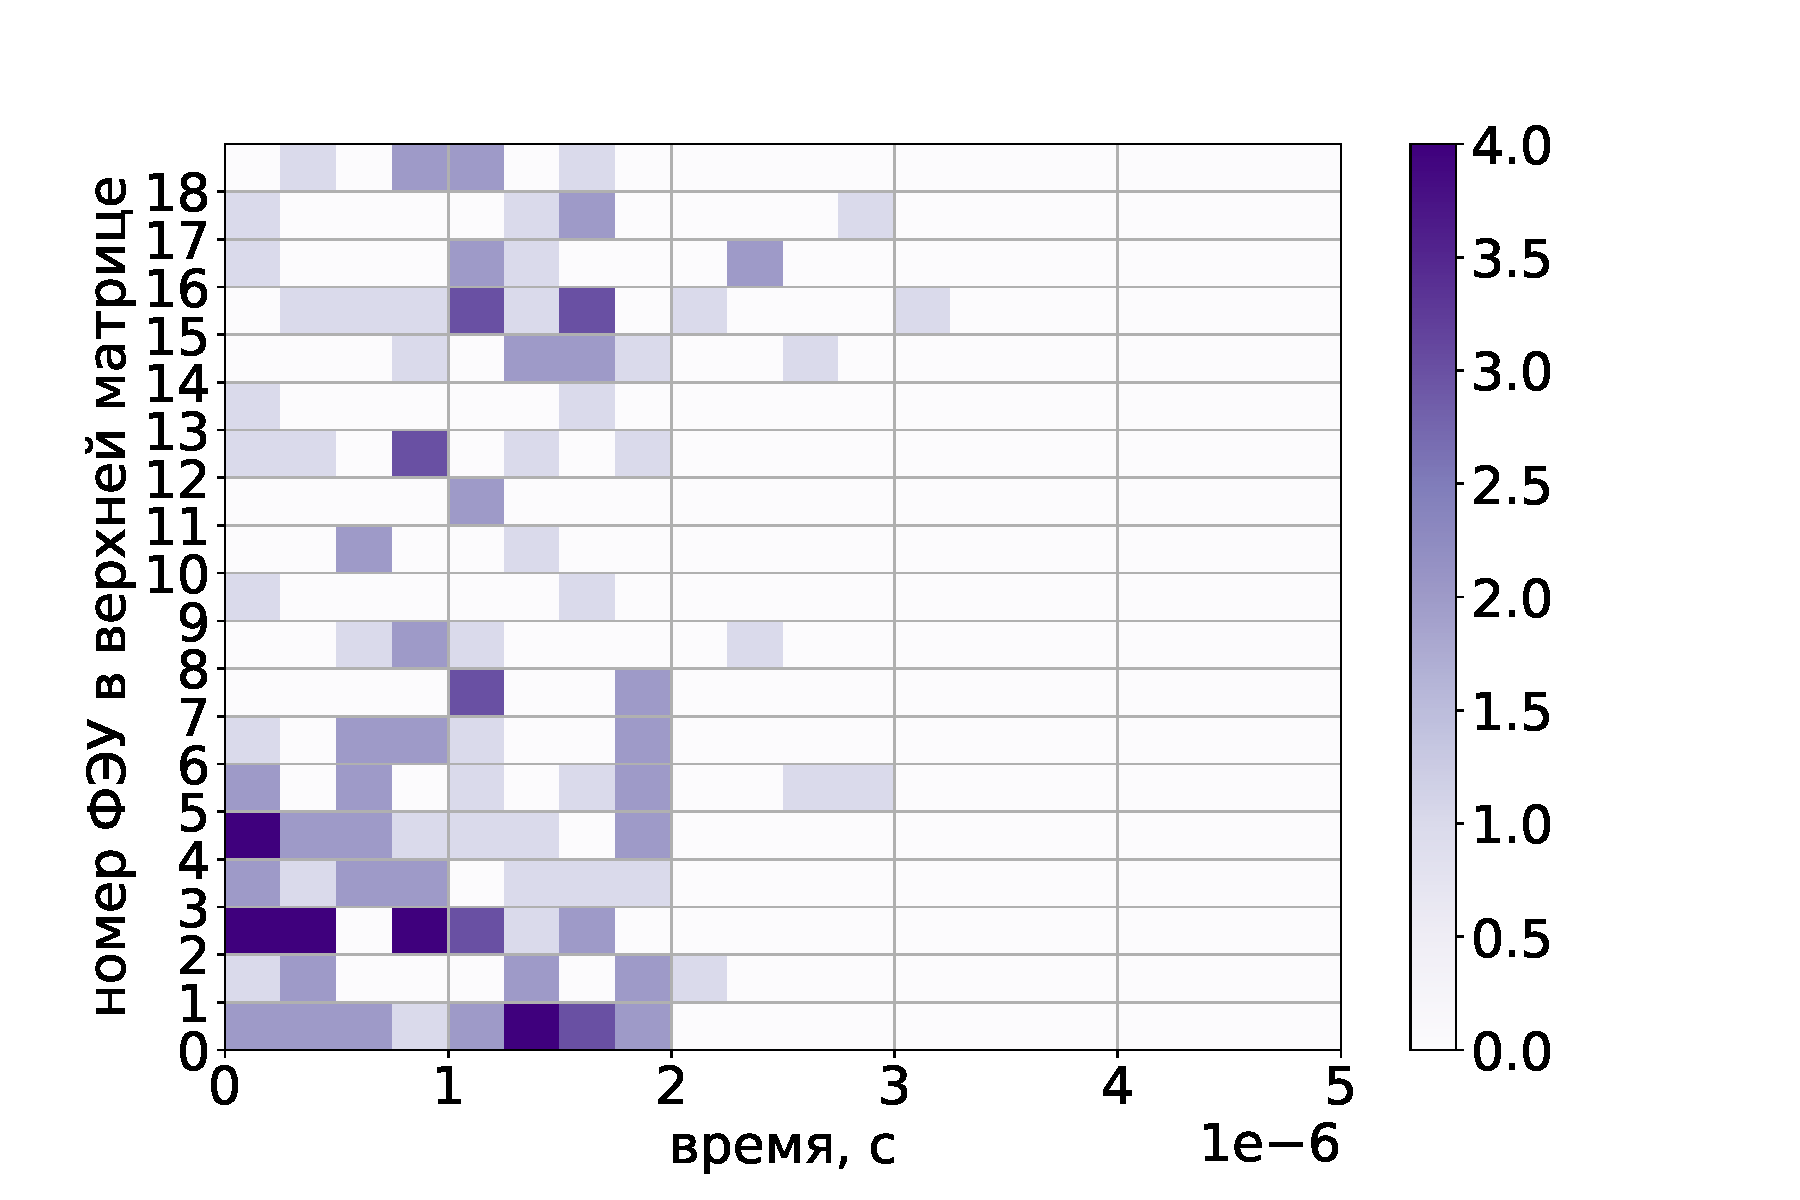
\includegraphics[width=1.0\linewidth]{images/bckg_event_6SE_1206_5.pdf} \\ б)}
  \end{minipage}
  \caption[Пример временных разверток смоделированных событий, применявшихся для тренировки нейросетей для отбора по точечности.]{Пример временных разверток смоделированных событий, применявшихся для тренировки нейросетей для отбора по точечности. a) -- точечное событие в 6 электронов ионизации, б) -- "неточечное" событие, состоящее из нескольних отдельных событий, в сумме дающих 6 электронов ионизации}
  \label{img:cevnsbckgevents}  
\end{figure}

\begin{table}[H]
    \centering
    \caption{Эффективности прохождения УКРН-событий для каждой из сетей, расчитанные по смоделированным данным.}  
\begin{tabular}{|c|c|c|c|c|}
\hline Количество SE & 3 & 4 & 5 & 6 \\
\hline сверточная сеть & $0.93$ & $0.96$ & $0.97$ & $0.98$ \\
\hline перцептрон & $0.88$ & $0.91$ & $0.93$ & $0.94$ \\
\hline
\end{tabular}
\label{NNeffcevns}
\end{table}

\begin{table}[H]
    \centering
    \caption{Эффективности подавления фоновых событий для каждой из сетей, расчитанные по смоделированным данным.}  
\begin{tabular}{|c|c|c|c|c|}
\hline Количество SE & 3 & 4 & 5 & 6 \\
\hline сверточная сеть & $0.87$ & $0.87$ & $0.93$ & $0.95$ \\
\hline перцептрон & $0.92$ & $0.93$ & $0.97$ & $0.98$ \\
\hline
\end{tabular}
\label{NNeffbckg}
\end{table}

Энергетический спектр фоновых событий до отборов по радиусу и точечности и после представлен на рисунке~\ref{img:bckgspecrtum}.
\begin{figure}[H]
\center{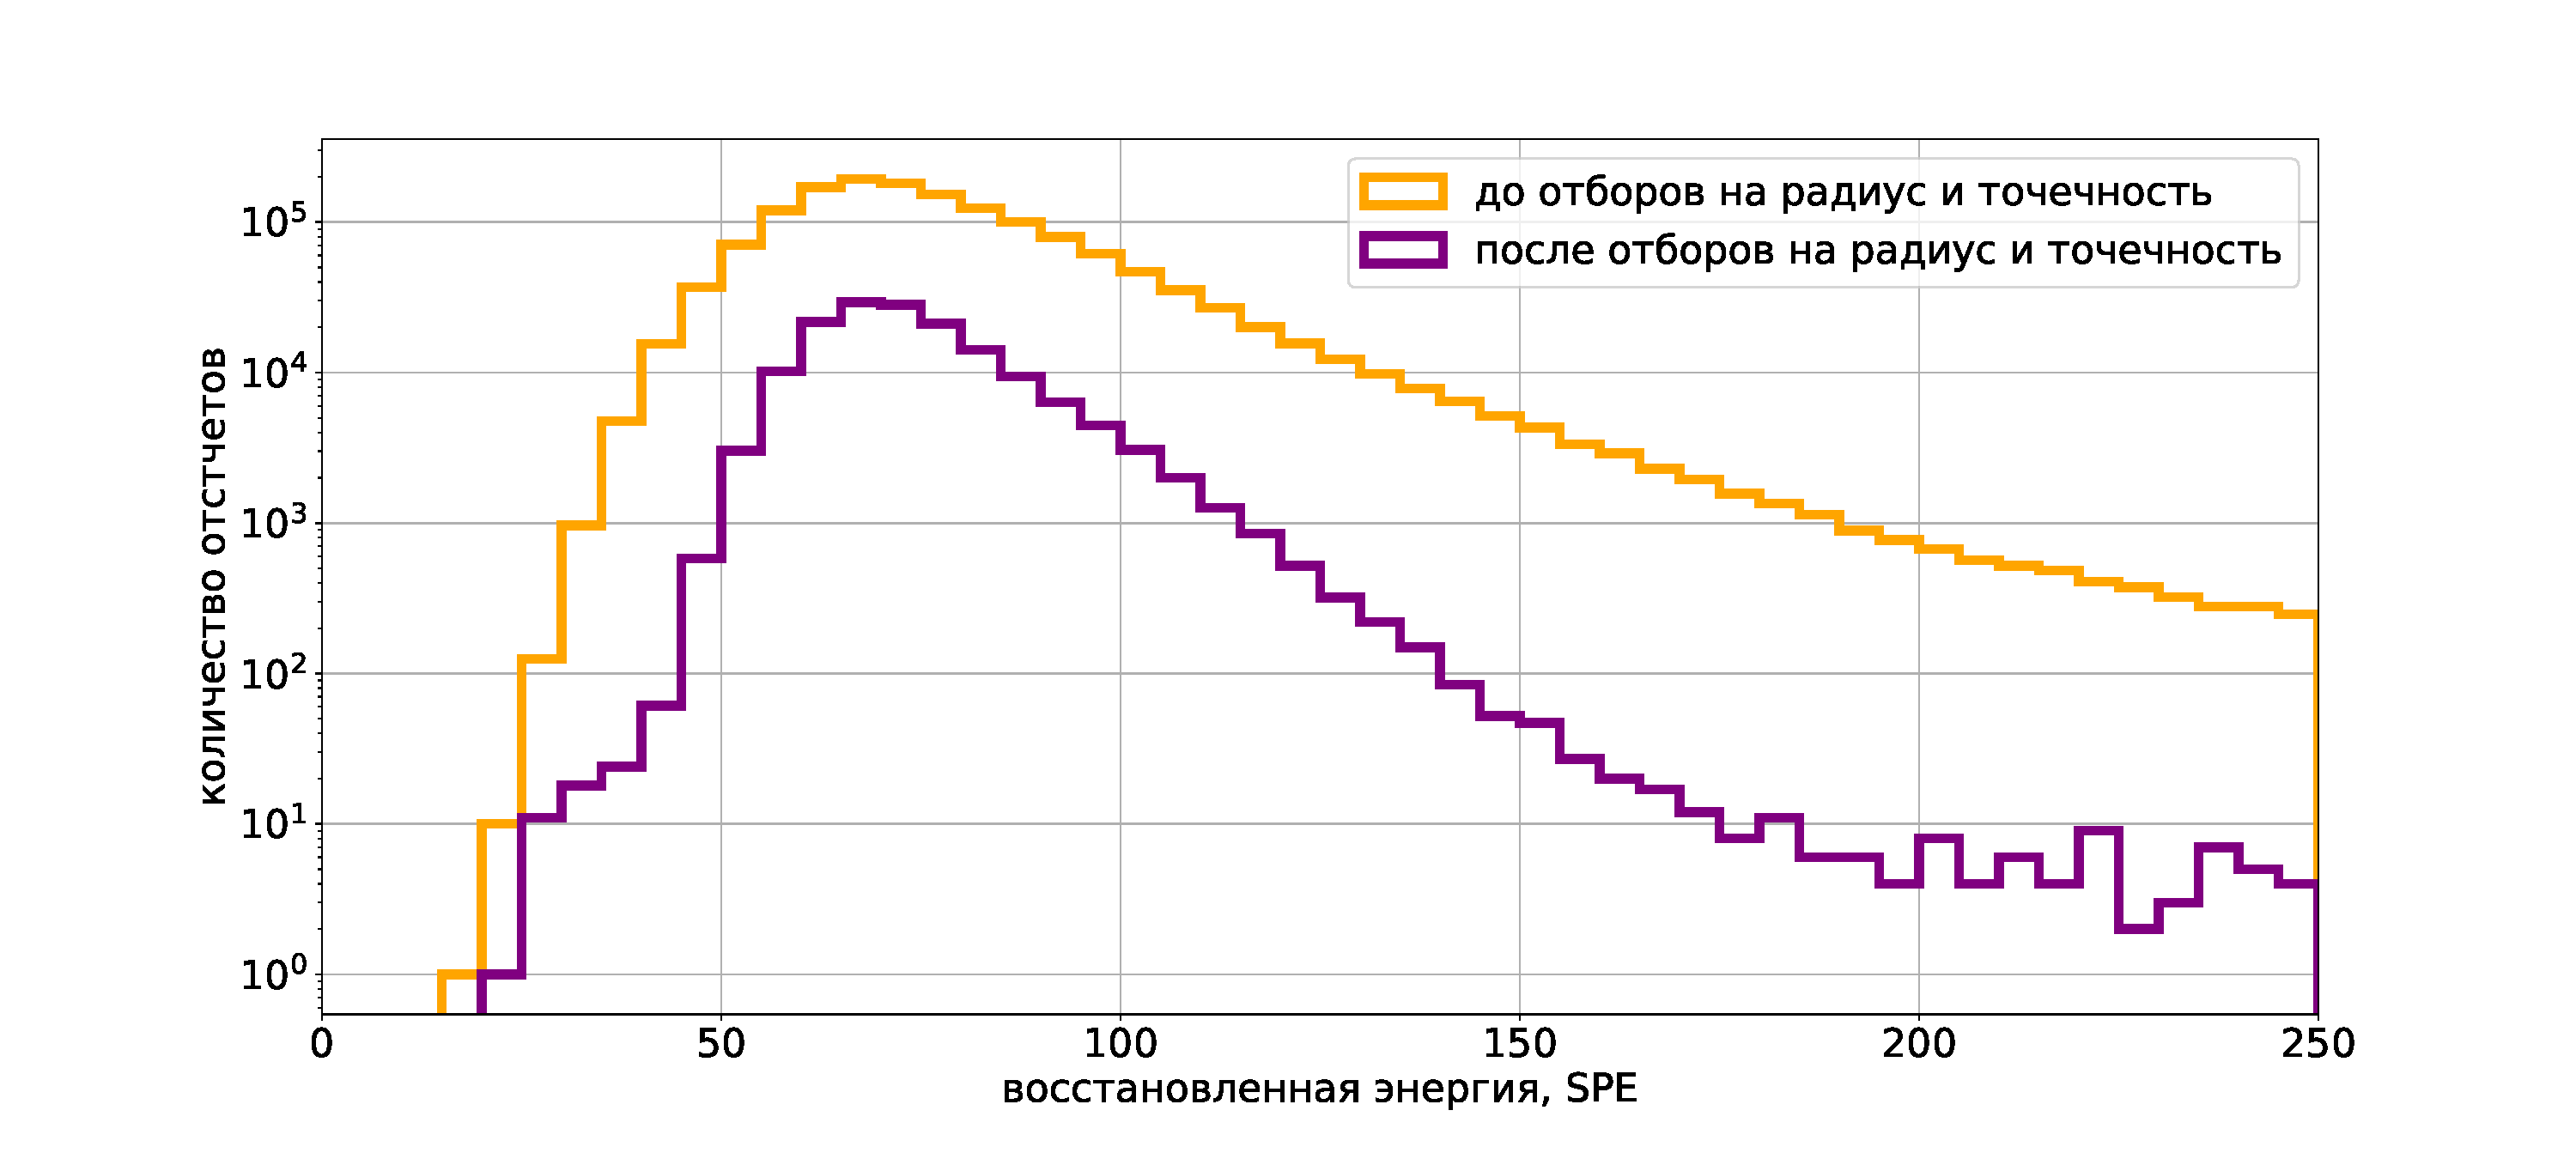
\includegraphics[width=0.8\linewidth]{images/cutsillustration.pdf}}
	\caption{Энергетический спектр фоновых событий до и после отборов по радиусу и точечности}
	\label{img:bckgspecrtum}
\end{figure}

%показать результирующий спектр
%заявить где-нибудь здесь живое время

\section{Анализ чувствительности}
\label{sect4_4}
Анализ чувствительности эксперимента РЭД-100 предполагает определение возможности обнаружения УКРН-событий с учетом фонового сигнала. При этом для улучшения результата проводится анализ не только количества событий, но и формы спектра. Также учитывается живое время набора данных с выключенным ($\sim$22 часа) и включенным ($\sim$73 часа) реактором.
Процедура, примененная для анализа чувствительности в данной работе, описана в~\cite{Matt_thesis}. Для анализа был использован трехмерный спектр, где по трем осям были отложены восстановленная энергия, длительность и восстановленный радиус. Общая идея метода состоит в определении количества событий УКРН, которые с определенной пороговой вероятностью не могут быть имитированы случайными флуктуациями фона.

%на основе экспериментального спектра
Для реализации данного метода на основе экспериментального спектра были сгенегированы 10000 наборов данных без сигнала, и для каждого набора данных было определено отношение правдоподобий:

\begin{equation}
   \Delta(-2 \ln L)_{N u l l} \equiv(-2 \ln L)_{N u l l}-(-2 \ln L)_{B F}
\label{likelihoodratio1}
\end{equation}

В данной формуле $(-2 \ln L)_{N u l l}$ -- значение логарифма функции правдоподобия в предположении нулевого количества событий, а $(-2 \ln L)_{B F}$ -- значение логарифма функции правдоподобия для наилучшего фитирования спектра физическим сигналом. 

Далее было определено значение $\chi^2_{c}$, как такое $\Delta(-2 \ln L)_{N u l l}$, для которого $x\%$ сгенерированных наборов данных имеют меньшее значение $\Delta(-2 \ln L)_{N u l l}$. В нашем случае значение $x\%$ было выбрано равным 90\%. Распределение $\Delta(-2 \ln L)_{N u l l}$ и значение $\chi^2_{c}$ показано на рисунке \ref{img:deltaloglikelihood}
%сказать что-нибудь на тему того, почему мы так лихо переходим от правдоподобия к хи-квадрат

\begin{figure}[H]
\center{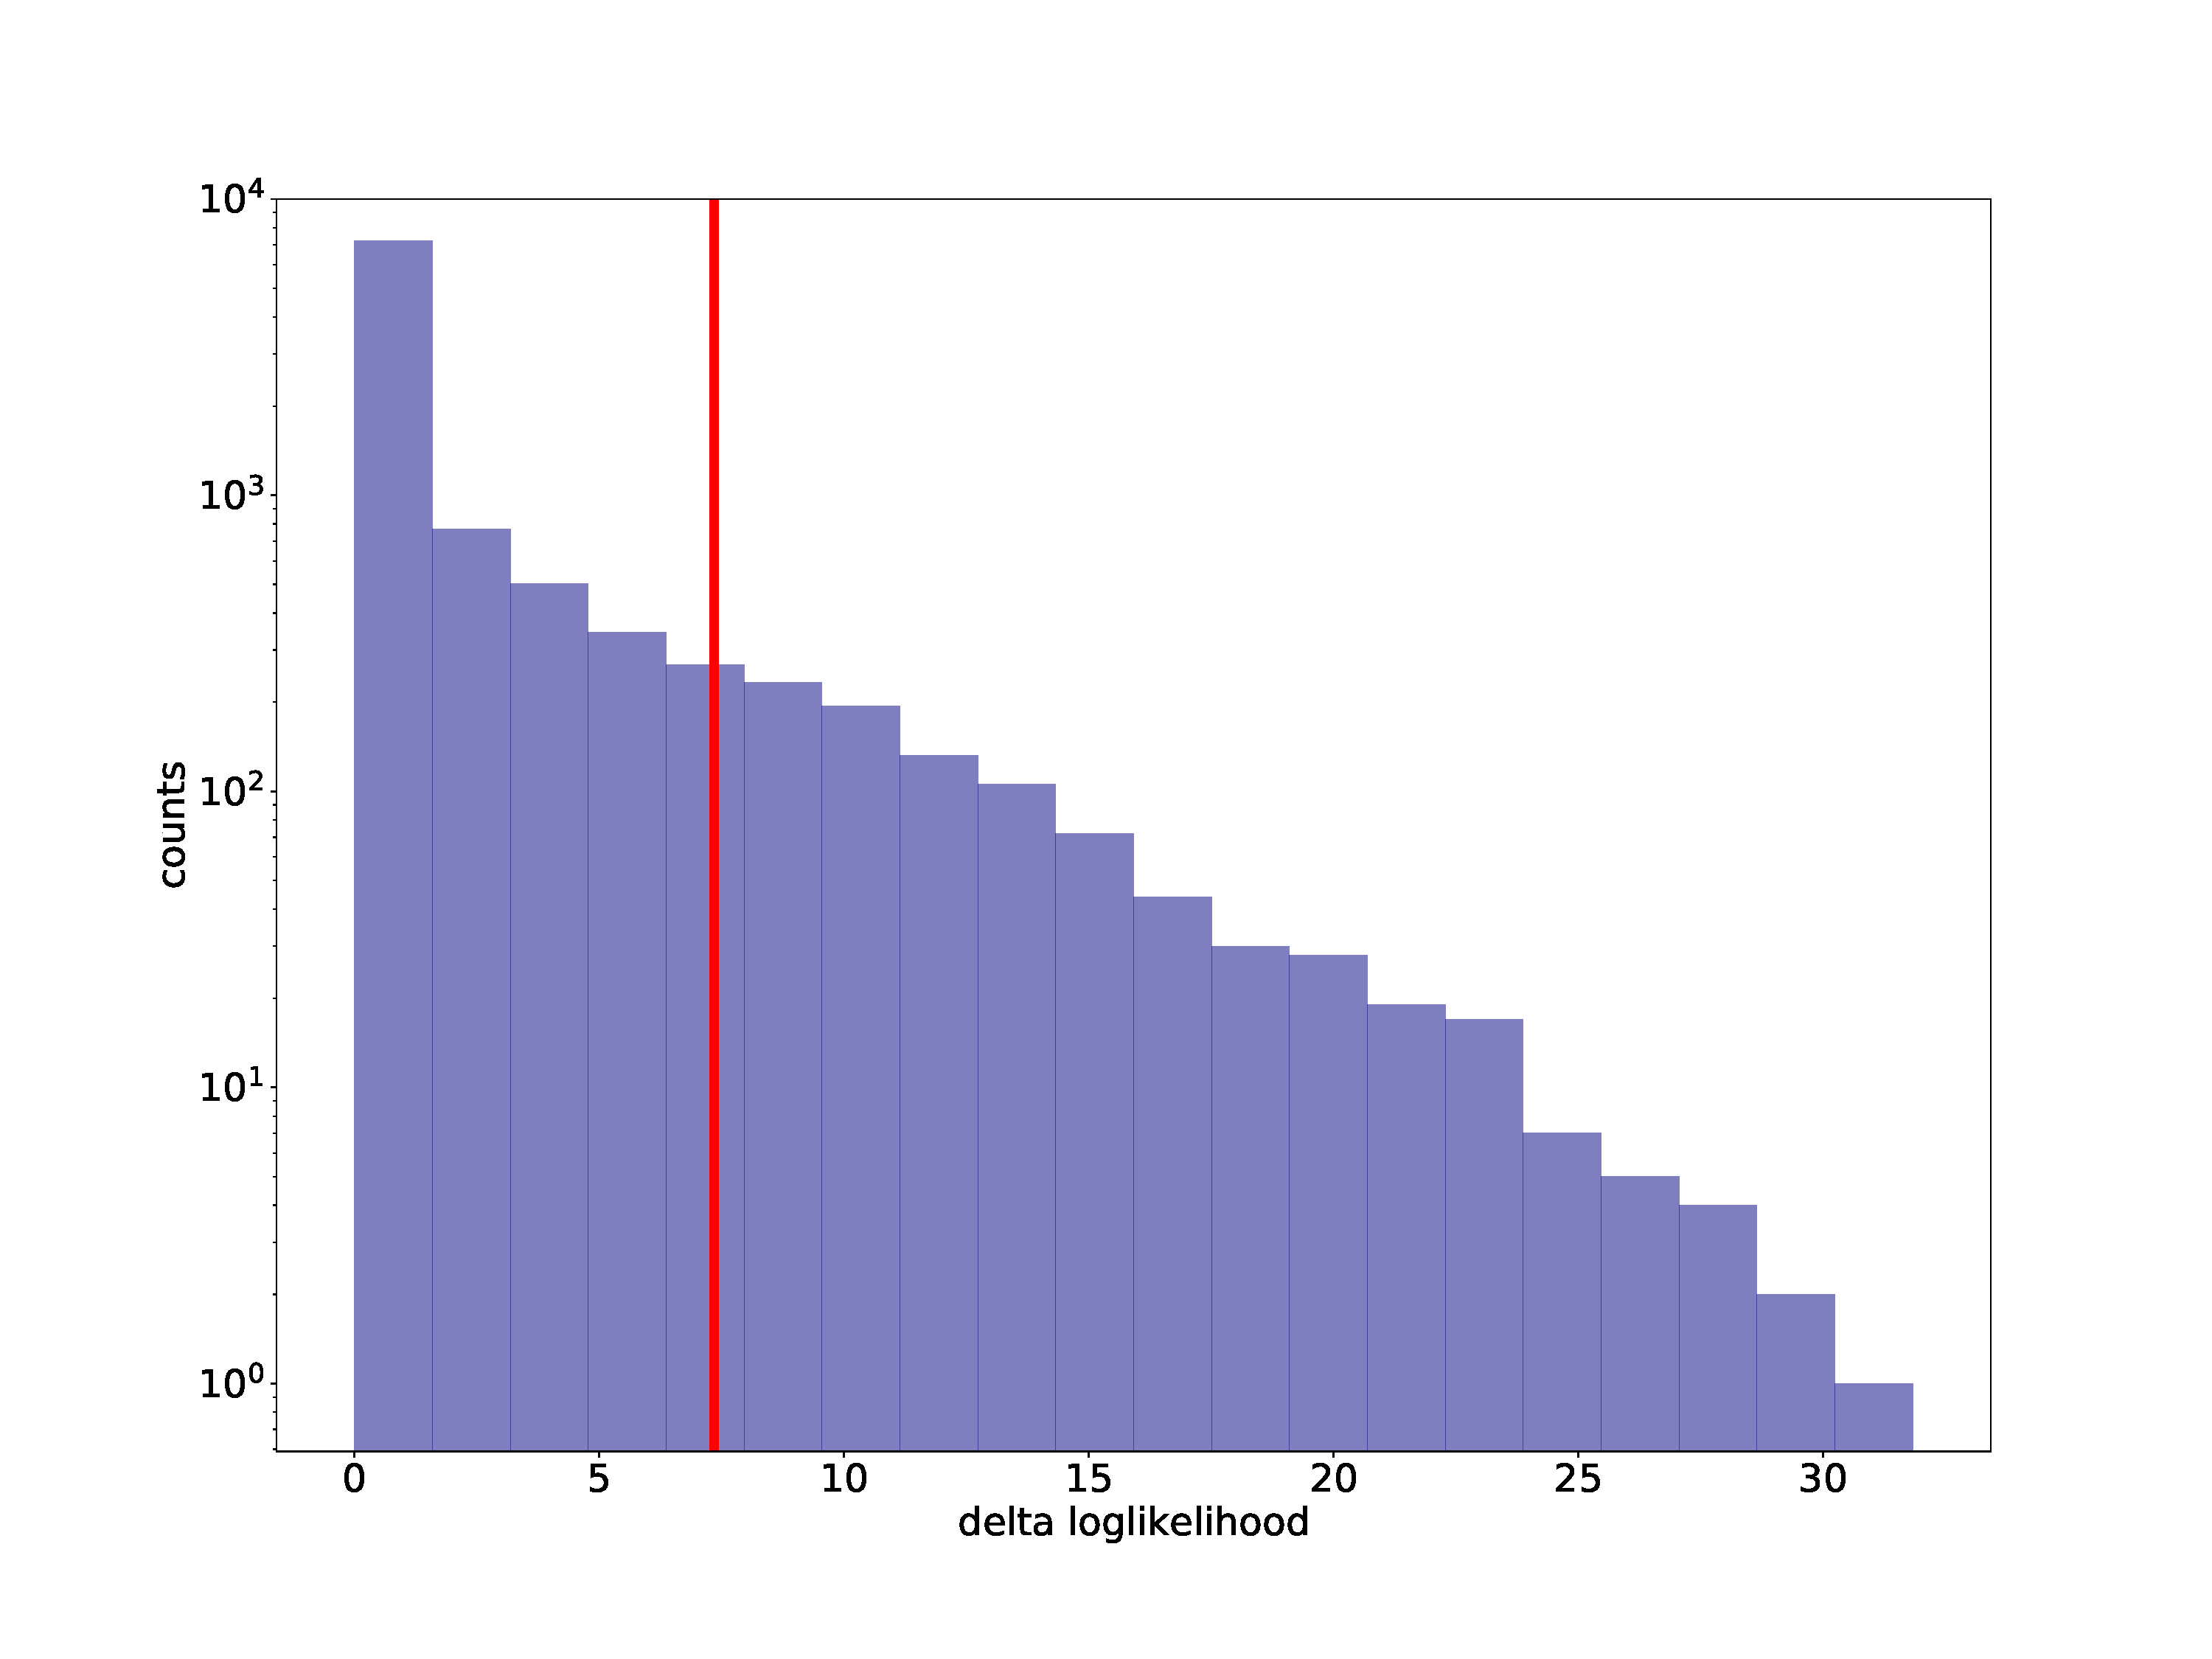
\includegraphics[width=0.8\linewidth]{images/deltaloglikelihood.pdf}}
	\caption{Спектр $\Delta(-2 \ln L)_{N u l l}$ для сгенерированных наборов данных. Красная линия показывает значение $\chi^2_{c}$.}
	\label{img:deltaloglikelihood}
\end{figure}

Далее для определения непосредственно чувствительности, были сгенерированы 3000 наборов данных, соответствующих определенному (варьируемому) количеству УКРН-событий в спектре. Для каждого уровня сигнала УКРН была определена доля ($\eta$) наборов данных с $(-2 \ln L)_{N u l l} > \chi^2_{c}$. Чувствительность определялась как количество УКРН событий, соответствующее набору с $\eta = 50\%$. Доля событий с $(-2 \ln L)_{N u l l} > \chi^2_{c}$ в зависимости от количества событий в день в области 5-6 электронов ионизации показана на рисунке \ref{img:rejectedsim}. 
%мб последнее предложение совместить с "для каждого..."
\begin{figure}[H]
\center{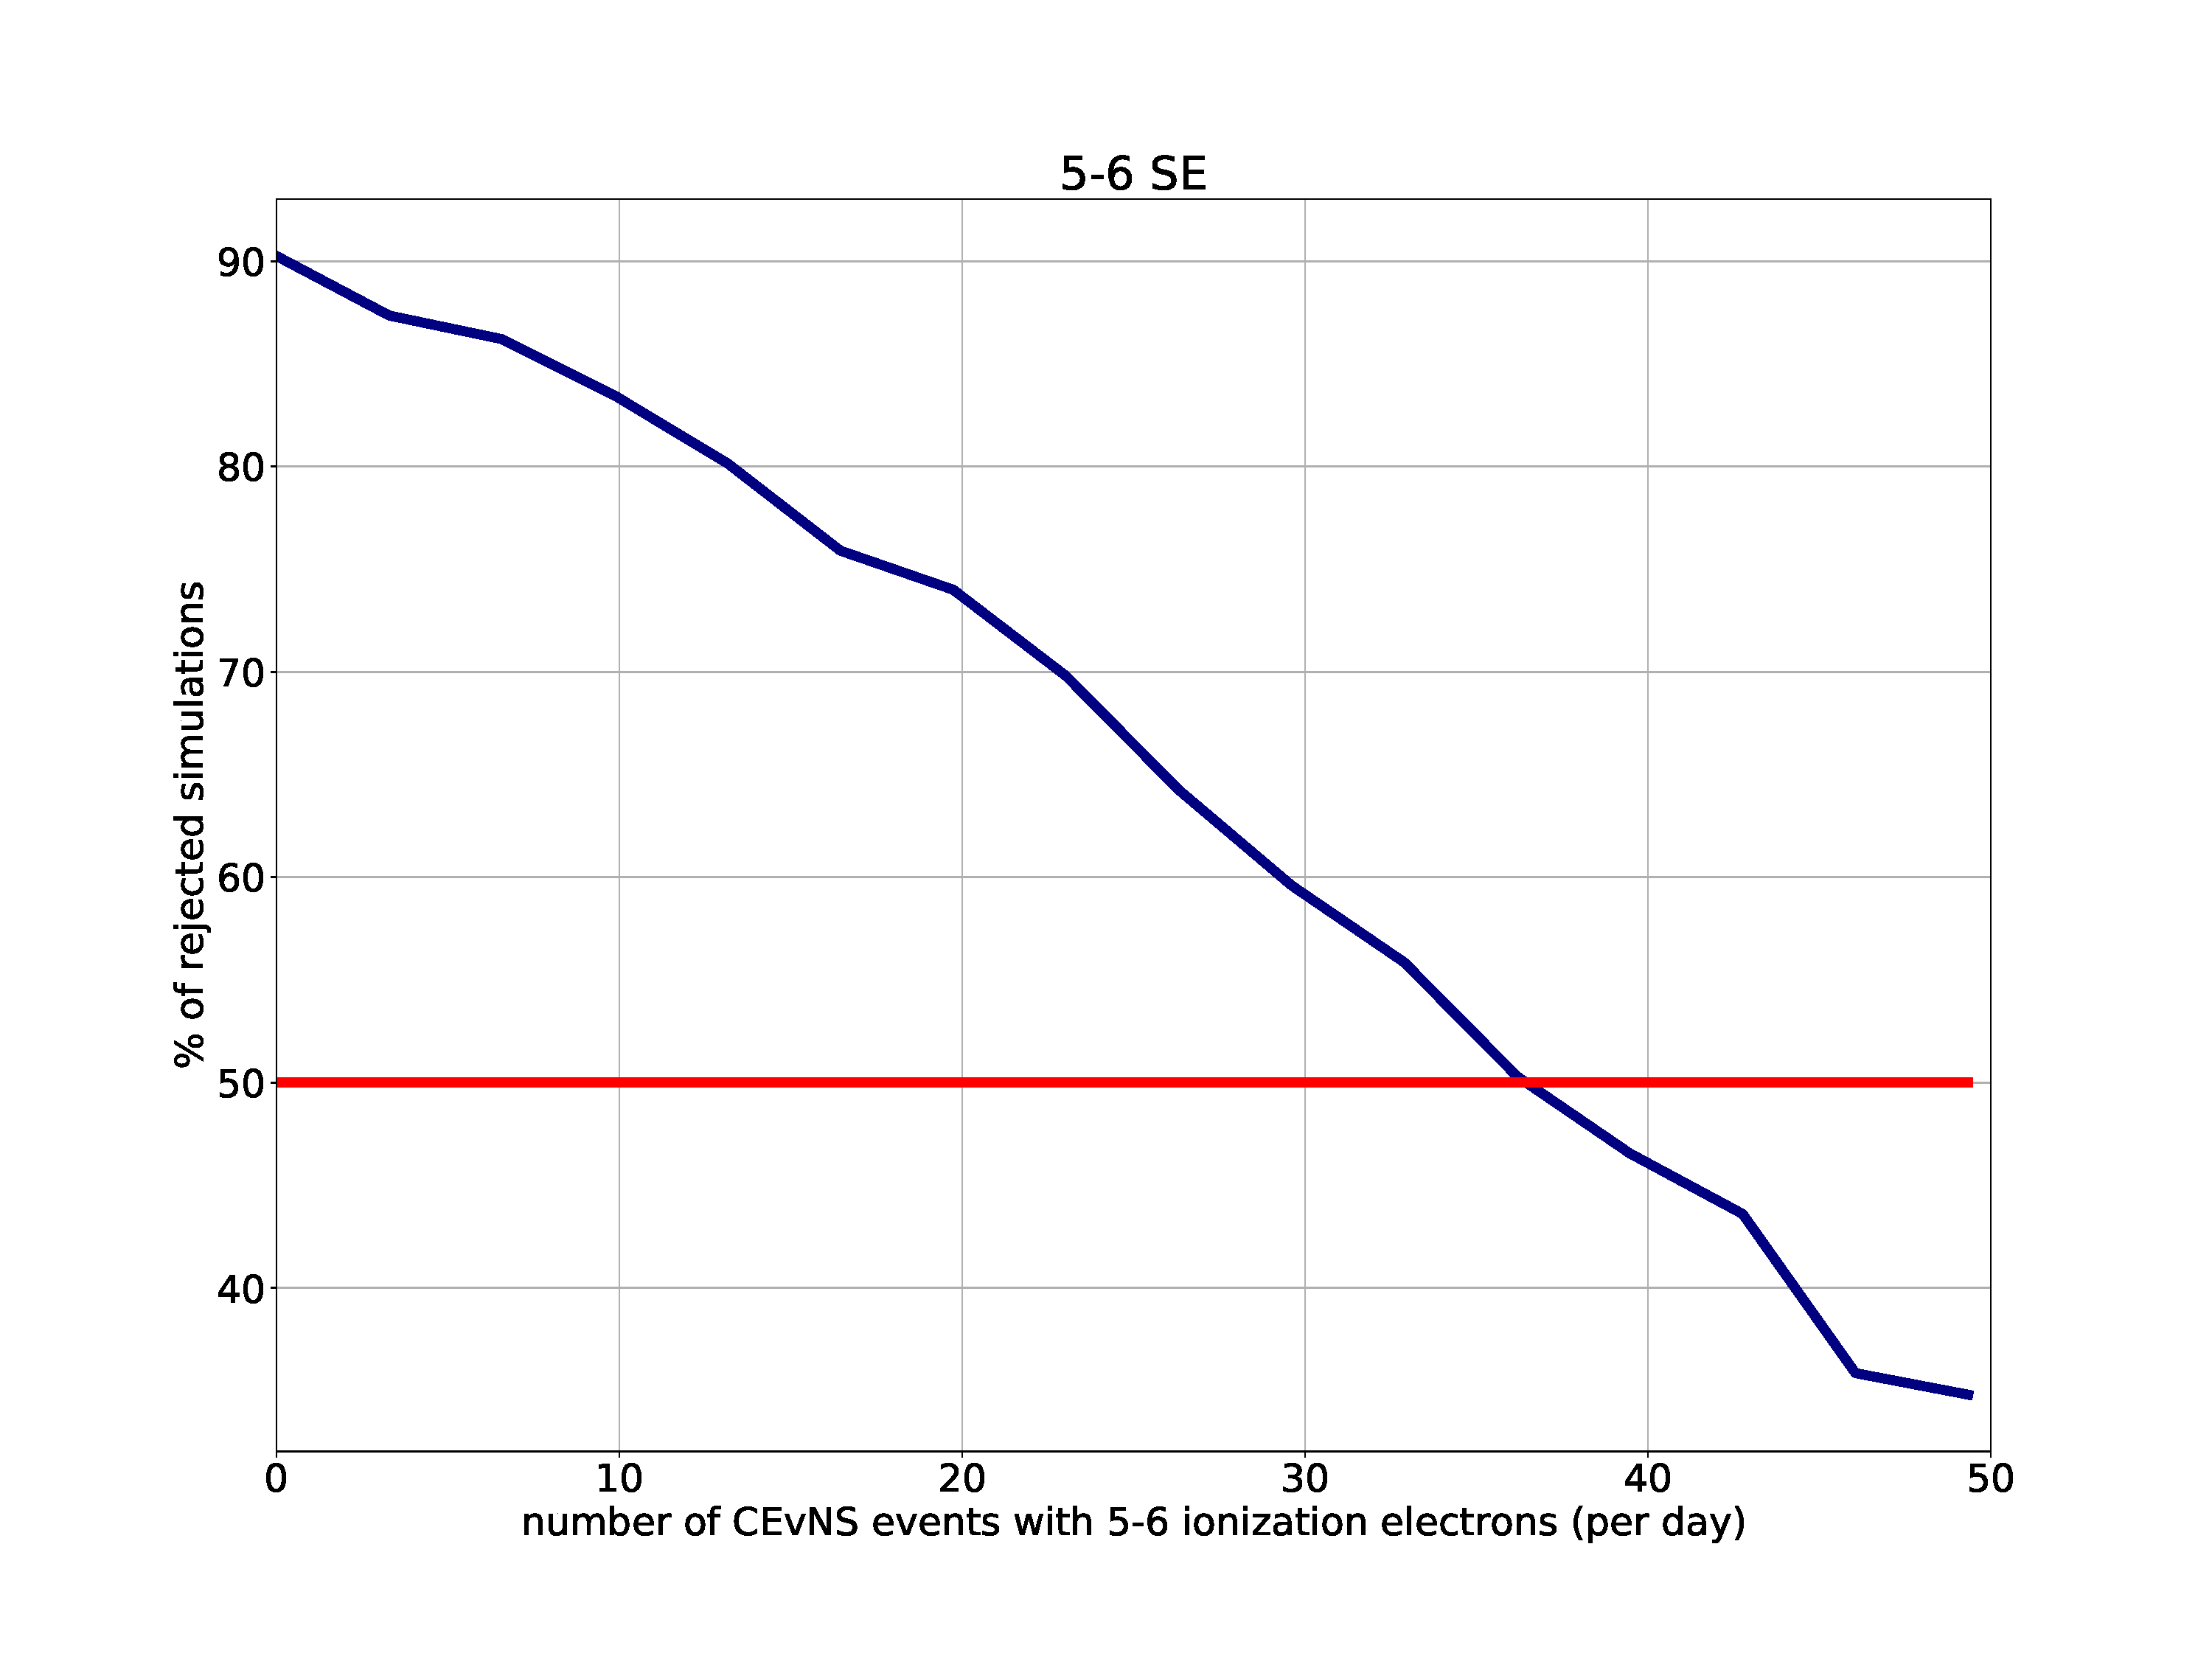
\includegraphics[width=0.8\linewidth]{images/rejected_simulations.pdf}}
	\caption{Доля событий с $(-2 \ln L)_{N u l l} > \chi^2_{c}$ в зависимости от количества событий в день в области 5-6 электронов ионизации. Красная линия показывает 50\%.}
	\label{img:rejectedsim}
\end{figure}

Полученное значение чувствительности ($\approx$37 событий УКРН в день) в $\approx$33 раз превышает предполагаемый уровень сигнала. Ожидаемое количество событий фона и сигнала приведено в таблице \ref{cevnscount}.

\begin{table}[hbt]
    \centering
    \caption{Ожидаемые скорости счета фона и сигнала (в день).}
    
\begin{tabular}{|c|c|c|c|c|}
\hline N e- & 3 & 4 & 5 & 6 \\
\hline bckg & $103 \mathrm{k}$ & $13.6 \mathrm{k}$ & 1268 & 150 \\
\hline CEvNS & $22.7$ & $4.7$ & $0.93$ & $0.19$ \\
\hline
\end{tabular}
\label{cevnscount}
\end{table}
